\documentclass[10pt,leqno]{article}
\usepackage[polish]{babel}
\usepackage[utf8]{inputenc}
\usepackage[T1]{fontenc}
\frenchspacing
%\usepackage{indentfirst}
\usepackage{listings}
\usepackage{framed}
\usepackage[textwidth=14cm,textheight=24cm]{geometry}
\usepackage{graphicx}
%\graphicspath{{img\\}}

\title{\LARGE Licencjacki projekt programistyczny 2011 \\ 
       \ \\
       Program do wykonywania obliczeń statystycznych związanych z grą go \\ 
       \ \\
       Podręcznik użytkownika }

% TODO autor wieksza czcionka

\author{Wojciech Jedynak}
\date{Wrocław, \today}

\newtheorem{rys}{Rysunek}

\begin{document}

\maketitle 

\thispagestyle{empty}
\tableofcontents

\newpage

\section{Wprowadzenie}

\subsection{Cel dokumentacji}
Zadaniem niniejszego podręcznika jest opisanie wszystkich aspektów dotyczących użytkowania programu GoStat od instalacji poprzez konfigurację
i eksploatację do jego deinstalacji.

\section{Wymagania}
Program najlepiej działa pod systemami linuksowymi. Instalacja dla systemów z rodziny Windows jest możliwa, ale wymaga większej liczby kroków. 

By używać programu konieczne jest posiadanie około 20 Mb miejsca na dysku oraz przeglądarki internetowej, która obsługuje JavaScript. 
W razie konieczności kompilacji programu należy posiadać połączenie z Internetem oraz udostępnić około 500 Mb dla kompilatora GHC (o ile nie 
został on już wcześniej zainstalowany).

\section{Instalacja i usuwanie programu}
Program jest dystrybuowany w dwu wersjach: w postaci binarnej oraz jako kod źródłowy.

\subsection{Postać binarna}
Należy: 
1) pobrać plik <GoStat-binary-os.tar.gz> (gdzie os to 'linux' bądź 'windows')
2) rozpakować archiwum do wybranego katalogu
3) przejść do ów folderu
4) uruchomić (najlepiej z poziomu terminala) plik GoStat (GoStat.exe w przypadku Windows)

W celu usunięcia programu wystarczy usunąć wymieniony wcześniej katalog oraz ew. wszystkie utworzone za jego pomocą bazy danych (pliki *.db).

\subsection{Kod źródłowy}
Należy:
1) rozpakować plik <GoStat-source.tar.gz>
2) przejść do katalogu GoStat
3) z poziomu terminala wydać polecenie <cabal install>
4) poczekać aż narzędzie cabal-install pobierze i zainstaluje wszystkie brakujące pakiety modułów Haskellowych (może to zająć do kilkunastu minut).

Jeśli instalacja przebiegnie pomyślnie program będzie dostępny po wydaniu polecenia <GoStat> (<GoStat.exe> dla Windows).

W celu usunięcia programu należy udać się do katalogu .cabal (domyślnie znajduje się on w katalogu domowym użytkownika) i usunuąć wszystkie
podfoldery, które w nazwie mają frazę <GoStat>. Ewentualnie skasować należy także wszystkie utworzone za pomocą programu bazy danych (pliki *.db).

\section{Uruchamianie i zamykanie programu}

\subsection{Rozpoczęcie pracy}
Aby rozpocząć pracę z programem należy wydać polecenie \\
<GoStat> \\ 
\\
Gdy program odpowie \\
<Listening on port 8000...> \\
należy otworzyć przeglądarkę internetową i wskazać adres \\
<http://localhost:8000> \\
\\
Powinna wówczas załadować się strona startowa:

\begin{rys}
\begin{center}
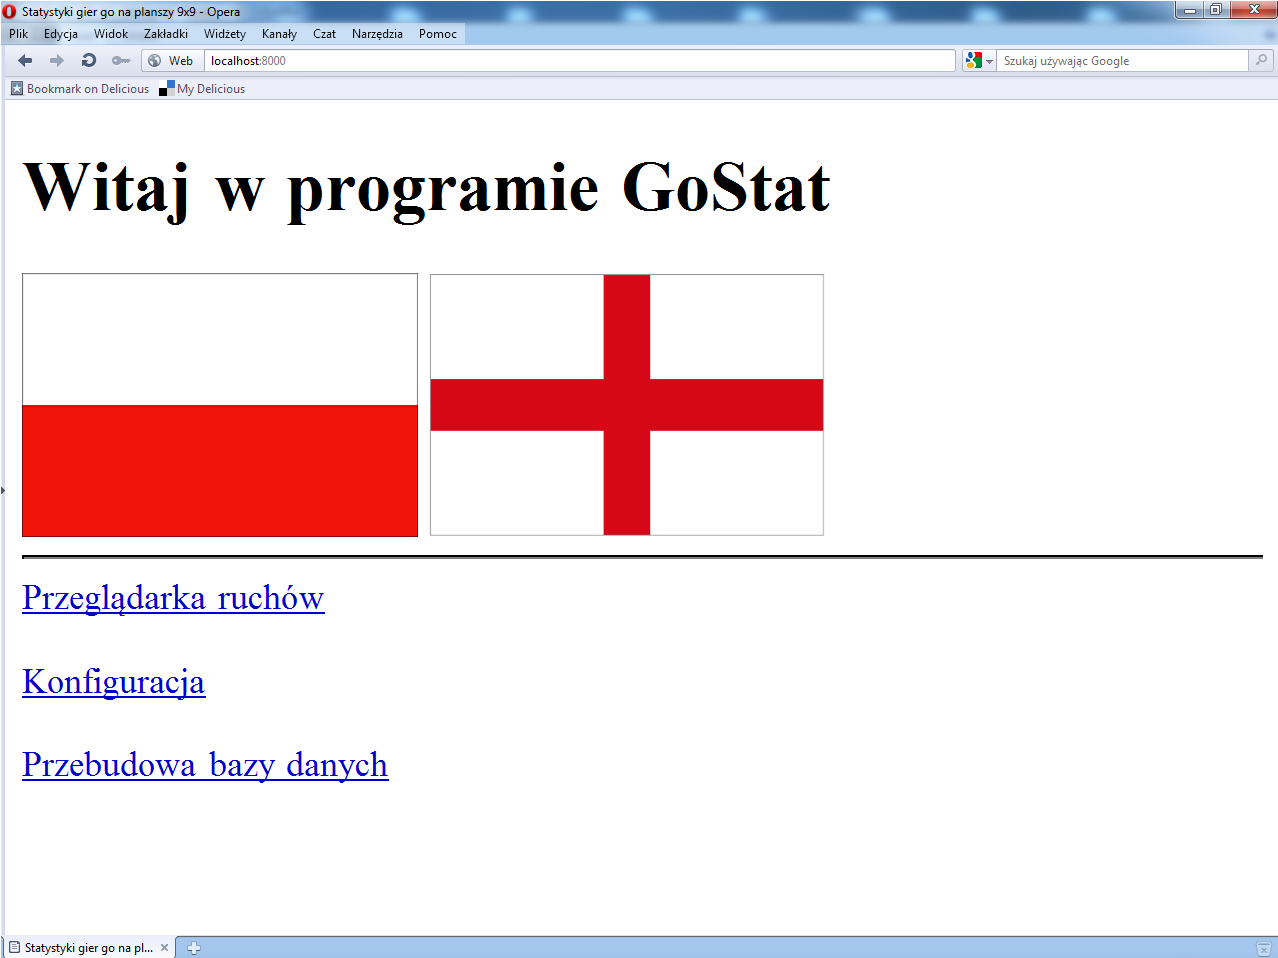
\includegraphics[scale=0.4]{start.png}
\end{center}
\end{rys}

\subsection{Kończenie pracy}
Aby zakończyć działanie programu należy zamknąć okno terminala bądź wysłać sygnał zakończenia (Control-C pod Linuks, Control-Z pod Windows).

UWAGA. Po wykonaniu tej czynności nie będzie można używać interfejsu WWW -- otrzymamy komunikat ``serwer nie odpowiada''. Aby przywrócić działanie programu
wystarczy go ponownie uruchomić.

\section{Konfiguracja programu}
Aby skonfigurować program, należy go: uruchomić (patrz rozdział: <Rozpoczęcie pracy>) i kliknąć odnośnik <Konfiguracja> widoczny na <Rysunku 1>.

Ukaże się wówczas następujący formularz:

\newpage

\begin{rys}
\begin{center}
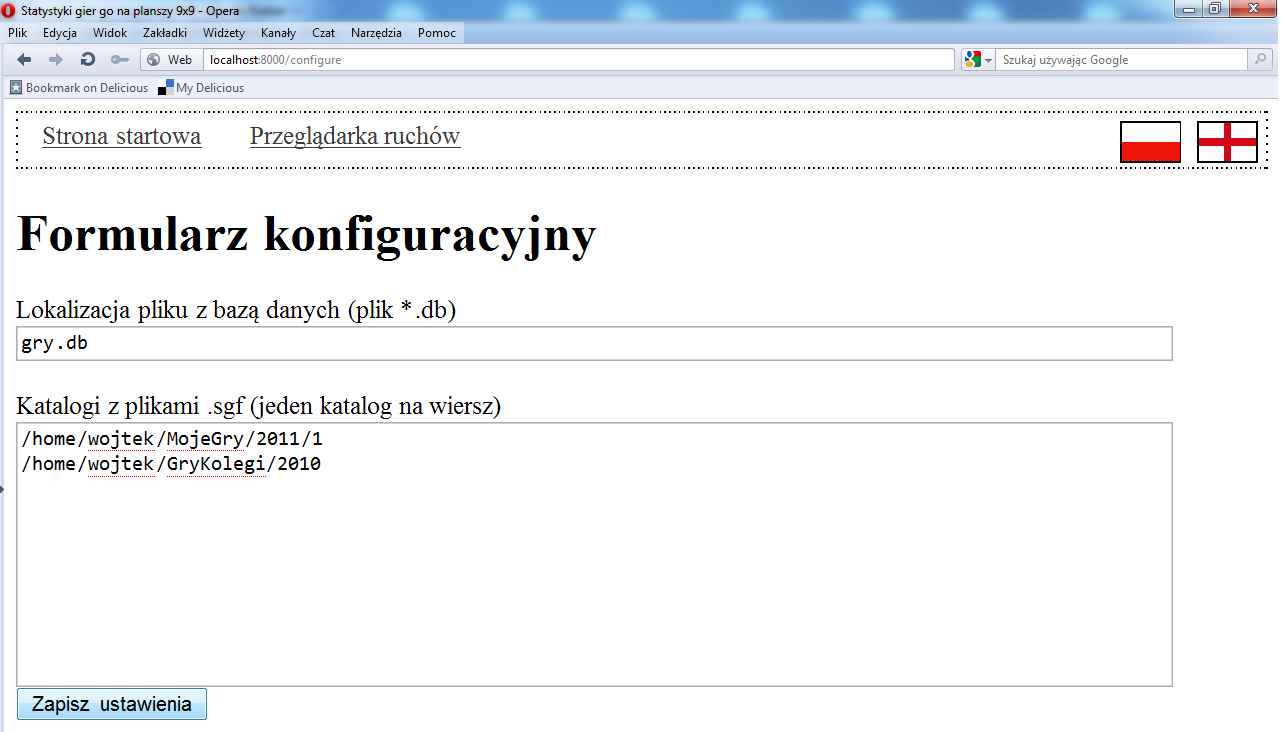
\includegraphics[scale=0.4]{formularz.png}
\end{center}
\end{rys}

Składa się on z dwóch pól tekstowych. 

W pierwszym z nich należy podać lokalizację pliku bazy danych o rozszerzeniu .db, którego GoStat użyje do zebrania informacji o podanych zapisach gier go.
Plik nie musi istnieć fizycznie na dysku -- zostanie on utworzony w razie potrzeby -- ale jeśli podany zostanie katalog, to wymagane jest, aby został on
wcześniej utworzony.

W drugim polu należy podać pełne (tj. bezwględne) scieżki do katalogów zawierających pliki .sgf z zapisami gier, które chcemy analizować przy pomocy
programu GoStat. W każdym wierszy pola tekstowego można podać osobną ścieżkę. \\
\textbf{Ważne:} nie trzeba podawać każdego katalogu osobno, gdyż program szuka gier we \textbf{wszystkich podkatalogach} podanych folderów.

Aby zapisać zmiany w konfiguracji, należy kliknąć <Zapisz ustawienia>. Wówczas automatycznie wrócimy do strony startowej (<Rysunek 1>). 
Aby wykonane zmiany były widoczne w przeglądarce ruchów, należy następnie wybrać <Przebudowa bazy danych>. Opcja ta jest opisana poniżej.

\section{Utworzenie i wypełnienie bazy danych}
Aby utworzyć (przebudować) bazę danych i wypełnić ją danymi, należy: 
  uruchomić program (patrz rozdział: <Rozpoczęcie pracy>)
  kliknąć odnośnik <Przebudowa bazy danych> widoczny na <Rysunku 1>.

Ponieważ przebudowa istniejącej bazy danych zaczyna się się od skasowania poprzedniej tabeli, użytkownik zostanie
poproszony o potwierdzenie swego zamiaru:

<potwierdzenie>

Po kliknięciu <OK> należy poczekać aż program wykona operację przebudowania do końca. 
Aby można było śledzić w czasie rzeczywistym postęp prac wyświetlona zostanie aktualizowana na bieżąco strona informacyjna:

<strona informacyjna>

Gdy wszystkie operacje zostaną wykonane, użytkownik zostanie automatycznie przekierowany do strony głównej (<Rysunek 1>).

\section{Praca z programem}
Nim wybierzemy <przeglądarka ruchów> należy skonfigurować program i utworzyć (ew. przebudować) bazę danych.

\subsection{Przeglądarka ruchów}

\section{Rozwiązania przykładowych problemów}

\end{document}
